\chapter{Desarrollo}

\section{Obtener datos satelitales y lecturas pluviom'etricas}

  La  \textit{National Oceanic and Atmospheric Administration} (NOAA) es una agencia federal Estadounidense que se encarga de 
  monitorear las condiciones oceanicas y atmosf'erica por medio de sus sat'elites.
  En particular los sat'elites geoestacionarios GOES 11 y 12 toman im'agenes en infrarrojo de las nubes que est'an sobre
  el territorio Mexicano.

  Para 'este proyecto pedimos a la NOAA que nos proporcionara informaci'on de una zona amplia del sur del pa'is en 
  intervalos de tiempo, en los cuales, se presentaron fen'omenos de importancia de inundaciones en la zona de Tabasco.

  Es necesario que se procese la información que se descarga directamente de los servidores de la NOAA. Para ello se usa
  una aplicaci'on llamada \textit{NOAAA Weather and Climate Toolkit} para generar archivos de texto plano que contienen
  toda la informaci'on de cada punto le'ido.

  \begin{figure}[h!]
  \centering
  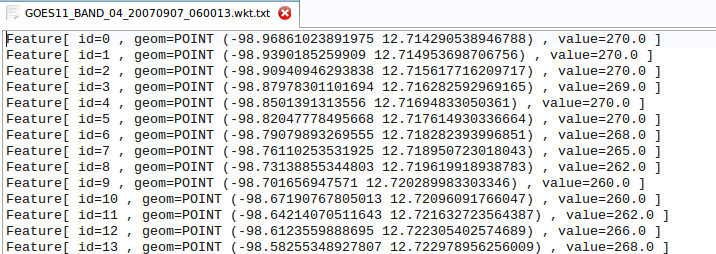
\includegraphics[width=170mm]{./imagenes/archivoTxt.png}
  % archivoTxt.png: 721x512 pixel, 72dpi, 25.43x18.06 cm, bb=0 0 721 512
  \caption{Archivo de informaci'on satelital en texto plano}
  \end{figure}


  La \textit{Comisi'on Federal de Electricidad} (CFE) posee una serie de estaciones de medici'on puvliom'etricas que registran 
  la lluvia que cae sobre la estaci'on en cada hora. El portal de la CFE permite acceder a las estaciones deseadas 
  y a las fechas disponibles. Desafortunadamente la informaci'on que provee la Comisi'on es limitada y en muchas 
  ocasiones incorrecta o incosistente.




\section{Dise\~no de la apliaci'on en C++/Fortran}
  %Porque se decidio usar C y Fortran
  Las aplicaciones que realizan c'alculos num'ericos complejos requieren que la velocidad de respuesta sea la m'inima posible y que
  la programaci'on de las mismas sea lo m'as sencilla.

  Hist'oricamente Fortran ha servido al mundo cient'fico para modelar sistemas complejos, su sint'axis, 
  muy similar al lenguaje matem'atico, lo hace sumamente atractivo para desarrollar aplicaciones num'ericas. Sin embargo,
  es su alta especializaci'on lo que permite al compilador hacer optimizaciones eficientes en el c'odigo, produciendo
  programas muy r'apidos.

  Por otra parte, C/C++ es un lenguaje de prop'osito general que permite al programador trabajar r'apidamente en tareas que requieren
  el uso de estructuras de datos y acceso a los servicios del sistema operativo. 
  En particular, el manejo de archivos, memoria y hacer conexiones a bases de datos.

  La combinaci'on de ambos lenguajes se realiza mediante la definici'on de m'etodos externos de C. De 'esta manera, es posible
  usar lo mejor de estos lenguajes obteniendo resultados eficientes usando una programaci'on sencilla.

  %Uso de un IDE

  Los entornos de desarrollo integrados (EDI) son herramientas sumamente 'utiles en la implementaci'on de proyectos de software.
  Los EDI son aplicaci'ones que consisten de un editor de c'odigo, un compilador, un depurador y una interfaz gr'afica.

  Para 'este proyecto se adopt'o Netbeans en su versi'on 7 pues es uno de los EDI m'as aceptados y f'aciles de usar. La integraci'on
  que posee con C y Fortran es limpia y sencilla.

  %uso de gitHub
  En cualquier proyecto de desarrollo de software es indispensable contar con un control de versiones del c'odigo. En particular,
  se opt'o por usar GitHub pues provee de una plataforma web robusta y sobre todo segura. Para 'este proyecto se uso un repositorio
  privado que garantiza que s'olo los colaboradores autorizados puedan ver y modificar el c'odigo.

  %Documentación usando doxygen
  La documentaci'on precisa del c'odigo se realiz'o mediante la herramienta doxygen. 'Esta herramienta sirve para generar
  documentaci'on autom'aticamente mediante el uso de comentarios especiales en el c'odigo. El producto final es una p'agina web, un manual 
  que puede ser visto con el comando man de UNIX y un documento PDF que detallan cada archivo, funciones y modulos usados en el sistema.
  

  Finalmente, existen dos bibliotecas que son utilizadas para realizar consultas
  a bases de datos MySQL. Una de ellas est'a implementada en C++ y la otra en C.
  Se eligi'o la biblioteca mysqlclient implementada en C por su facilidad de uso.

\subsection{Estandarizaci'on de la informaci'on}
  %Mallas artificiales
  Uno de los primeros problemas al manejar la informaci'on del sat'elite fue la naturaleza de la informaci'on 
  misma. 

  Los sat'elites GOES 11 y 12 entregaban im'agenes con resoluciones diferentes y, por lo tanto, puntos 
  diferentes para la misma hora; m'as a'un, las im'agenes no presentaban necesariamente una forma regular.

  El primer paso para manejar de manera confiable la informaci'on fue realizar un pre-proceso de la misma
  de tal manera que se contara con im'agenes consistentes y regulares.

  La soluci'on adoptada fue dividir el territorio nacional en intervalos establecidos para generar una malla regular
  a la cual se podía ajustar la informaci'on de los satélites.

  Una vez definida la malla, se subi'o su informaci'on a la base de datos para poder obtener 
  de manera din'amica los puntos que se deben considerar para cualquier poligono. 

  El siguiente paso fue implementar un algoritmo de interpolaci'on que tomara una im'agen satelital arbitraria y 
  ajustara su informaci'on a una malla contenedora.

  C'omo se ilustra en la Figura 2.1, la informaci'on del satélite puede ser muy irregular. Para resolver el problema 
  envolvemos la im'agen en la malla e interpolamos la informaci'on. Las zonas para las cuales no hay datos disponibles
  son rellenadas de valores -1 (Se acord'o que un valor negativo para las lluvias sería un buen indicador de que no hay
  informaci'on).

  %%Hacer una imagen de como podría estar la imágen satelital y como se encierra dicha im'agen en una malla artificial
  \begin{figure}[h!]
  \centering
  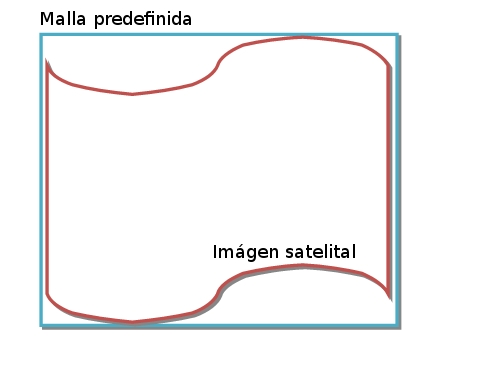
\includegraphics[width=120mm,bb=0 0 502 388]{./imagenes/malla.jpg}
  % malla.jpg: 502x388 pixel, 72dpi, 17.71x13.69 cm, bb=0 0 502 388
  \caption{Interpolaci'on de las imagenes satelitales}
  \end{figure}

  El programa de interpolaci'on fue implementado en Fortran mientras que las subrutinas para 
  pedir la malla adecuada a la base de datos fue implementada en C.

\subsection{Descripci'on del argoritmo STAR}
  El algoritmo STAR se encarga de transformar las temperaturas registradas por los sat'elites y las convierte
  en una primer estimaci'on pluvial. Recibe como entrada una matr'iz de temperaturas y para cada punto $p$ de la matr'iz
  obtiene una vecindad de radio $50$ alrededor del punto. Para 'esta vecindad calcula la media $prom$ y la desviaci'on estandard $\sigma$.

  Usando 'esta informaci'on se calculan dos 'indices llamados $RRn$ y $RRc$ que finalmente son utilizados por el algoritmo STAR

  \begin{algorithm}
  \caption{C'alculo del 'indice RRc}

  \begin{algorithmic}
  \IF {$temperatura \geq 201$}
	  \STATE $rrc \gets 1.1183* (100000000000.0)^(-0.036382*temperatura^{1.2})$
  \ELSE
	  
	  \STATE $rrc \gets 72$ \COMMENT{m'aximo valor de lluvia posible}
	  
  \ENDIF 
  \end{algorithmic}
  \end{algorithm}

  \begin{algorithm}
  \caption{C'alculo del 'indice RRn}

  \begin{algorithmic}
  \IF {$temperatura \geq 250$}
	  \STATE $rrn \gets 0$
  \ELSE
	  
	  \STATE $rrn \gets min(\frac{250-temp}{5}, 12)$ 
	  
  \ENDIF 
  \end{algorithmic}
  \end{algorithm}

  \begin{algorithm}
  \caption{Algoritmo STAR}

  \begin{algorithmic}
  \FOR{cada punto en la imagen}
      \STATE $vecindad \gets VecindadRadio50(x,y)$
      \STATE $prom \gets Promedio(vecindad)$
      \STATE $sigma \gets Desviacion(vecindad)$  
      \STATE $rrc \gets ComputarRRc((x,y).precipitacion)$
      \STATE $rrn \gets ComputarRRn((x,y).precipitacion)$
      \STATE $z = min(\frac{prom-(x,y).precipitacion}{sigma}, 1.5)$
      \IF { $z > 0$}
	\STATE $rr = \frac{rrc*z^2 + rrn*(1.5-z)^2}{z^2+ (1.5-z)^2}$
      \ELSE	  
	\STATE $rr = 0$   
      \ENDIF
    \ENDFOR
  \end{algorithmic}
  \end{algorithm}

Es importante mencionar que 'este proceso se ejecuta para cada lectura del sat'elite. Es posible que se tengan 3 o 4 lecturas por hora. El algoritmo 
Asimilaci'on requiere que se tenga una sola lectura por hora. Es entonces que se debi'o realizar un promedio de los archivos si se tienen dos lecturas y 
ejecutar un algoritmo trimean cuando se tengan 3 lecturas. De 'esta manera se conserva el mejor valor posible para cada hora.

\subsection{Descripci'on e implementaci'on del algoritmo Asimilaci'on}
El algoritmo Asimilaci'on realiza una serie de pasos que se detallan a continuaci'on:
\begin{enumerate}
 \item Descargar la malla predefinida para el pol'igono definido por el usuario.
  \item Computar el algoritmo STAR para obtener \textbf{hasta} 3 horas previas de la que se desea calcular.
  \item Completar la informaci'on del paso anterior con -1 en donde no se encuentre informaci'on usando la malla predefinida del paso 1.
  \item Descargar las lecturas de las estaciones que se ubican dentro del pol'igono.
  \item Correr el algoritmo \textbf{Asimilaci'on-Fortran}.
  \item En caso de 'exito, subir la informaci'on nueva a la base de datos y graficarla
  \item En caso de fracaso (informaci'on insuficiente), se debe graficar s'olo la informaci'on del algoritmo STAR.
  \item Correr el an'alisis de error puntual para cada estaci'on dentro del pol'igono.
\end{enumerate}
 %Falta describir el algoritmo Asimilacion-Fortran

\subsection{Productos generados}
%archivo de precipitacion .debug
\subsubsection*{Archivo de lluvia}
El programa genera un archivo con terminaci'on .debug que contiene la informaci'on calculada de las lluvias.
'Este archivo puede ser leído por programas de graficaci'on como gnuplot y matlab para su análisis.

En la Figura 2.2 podemos observar un ejemplo de un archivo .debug. 'Este archivo
consta de una cabecera que define las esquinas de la pol'igono y una lista de vectores (x, y, precipitación). La
lista de vectores define una matr'iz regular ordenada por renglones.

\begin{figure}[h!]
 \centering
 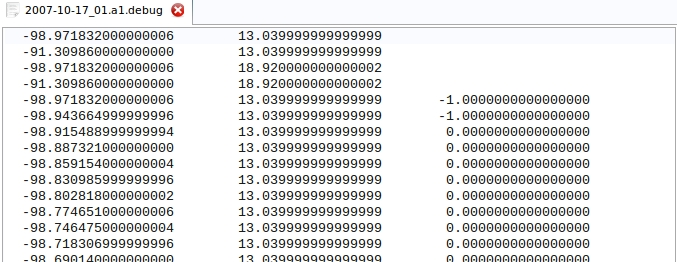
\includegraphics[width=160mm,bb=0 0 677 262]{./imagenes/archivodebug.jpg}
 % archivodebug.jpg: 677x262 pixel, 72dpi, 23.88x9.24 cm, bb=0 0 677 262
 \caption{Archivo de lluvia}
\end{figure}

\subsubsection*{Archivo de estimaci'on puntual}
%archivo de estimaci'on puntual
El archivo de estimaci'on puntual describe el comportamiento de los 2 algoritmos de estimaci'on pluvial y los compara
contra la precipitaci'on real reportada por las estaciones de la CFE.

El archvio de estimaci'on puntual es un archivo .csv que contiene los siguientes campos por estaci'on: 
\textbf{Nombre de la estaci'on, longitud, latitud , Valor real, Valor rain rate, Valor asimilado}

El objetivo de 'esta tabla consiste en generar inicialmente diagramas de dispersi'on como el mostrado en la Figura 2.3:

\begin{figure}[h!]
 \centering
 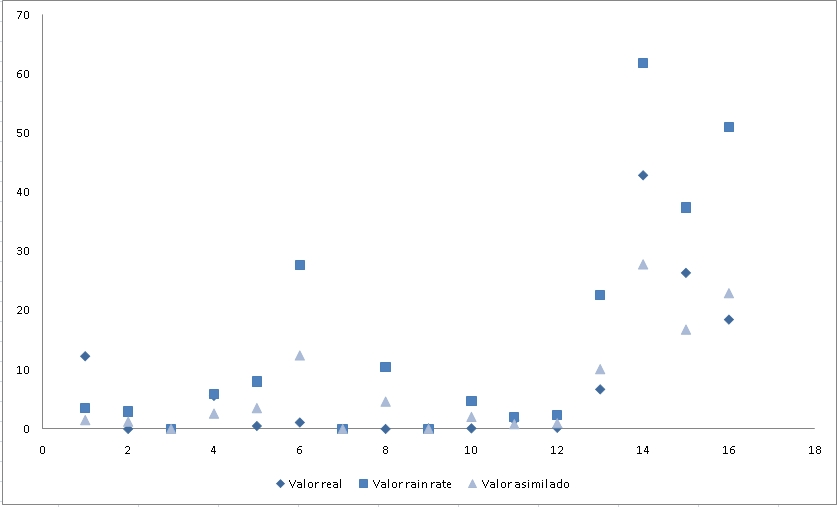
\includegraphics[width=170mm,bb=0 0 837 507]{./imagenes/archivoErrorAnalysis.png}
 % archivoErrorAnalysis.jpg: 837x507 pixel, 72dpi, 29.53x17.89 cm, bb=0 0 837 507
 \caption{Diagrama de dispersi'on}
\end{figure}

En la figura 2.3 se muestra un diagrama de dispersi'on de las predicciones realizadas en cada paso ejecutado por el sistema.
En el eje ${y}$ se representa la precipitaci'on en una hora en particular, 
en el eje $x$ son representadas las estaciones que caen dentro de un poligono
determinado. 


%archivo de error sigma desv esta
\subsubsection*{Mapas de lluvia}

Para poder presentar una im'agen de la estimaci'on pluvial probamos diferentes programas de graficaci'on, entre los cuales
destacan gnuplot y grads.

Se eligió usar GrADS, dise\~nado originalmente por \textit{ NASA Advanced Information Systems Research Program}, 
pues es un programa de propósito específico para manipular y visualizar datos generados por las Ciencias 
de la Tierra. Por otra parte, gnuplot es un programa de uso generar para graficar gran variedad de datos cient'ificos, lo cual
lo hace poco eficiente para graficar nuestra informaci'on, en particular, el uso de curvas de nivel fue privativo en tiempo
de ejecuci'on y en nivel de detalle de la im'agen.

Se puede apeciar en la figura que GrADS nos permite integrar la informaci'on de ubicaci'on y estado de las estaciones,
mostrando en rojo las estaciones que no poseen informaci'on, en verde las que si la poseen y en amarillo las que 
tienen informaci'on incompleta.

Directamente la im'agen generada por GrADS es un archivo eps \textit{Encapsulated PostScript}, sin embargo a pesar de la buena calidad
de las im'agenes eps, se debi'o convertir en formato jpg para conservar la compatibilidad con los navegadores web.

\begin{figure}[h!]
 \centering
 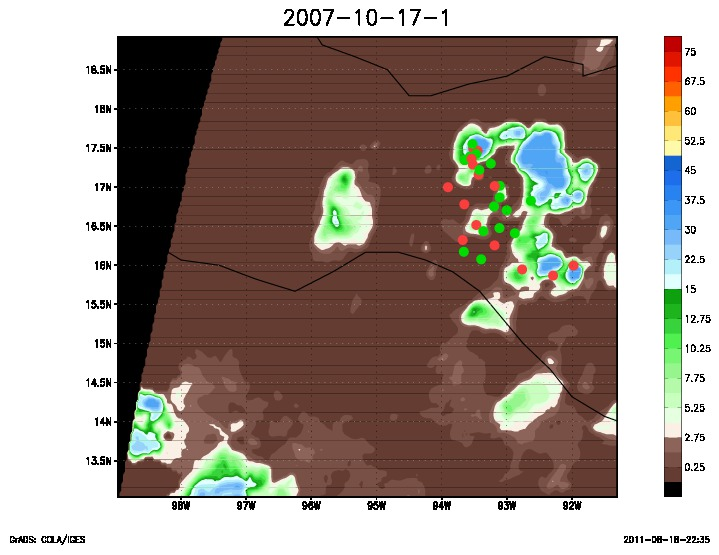
\includegraphics[width=120mm]{./imagenes/2007_10_17_1.jpg}
 % 2007_10_17_01.eps.jpg: 719x555 pixel, 72dpi, 25.36x19.58 cm, bb=0 0 719 555
 \caption{Im'agen generada por GrADS de la ventana completa de datos}
\end{figure}

La generaci'on de im'agenes fue de vital importancia para poder notar detalles desicivos entre una cantidad enorme de datos.
El uso de im'agenes nos permiti'o observar que las im'agenes satelitales que provee la \textit{NOAA} abarcaban una zona mucho
m'as peque\~na que la que se solicit'o.

\begin{figure}[h!]
 \centering
 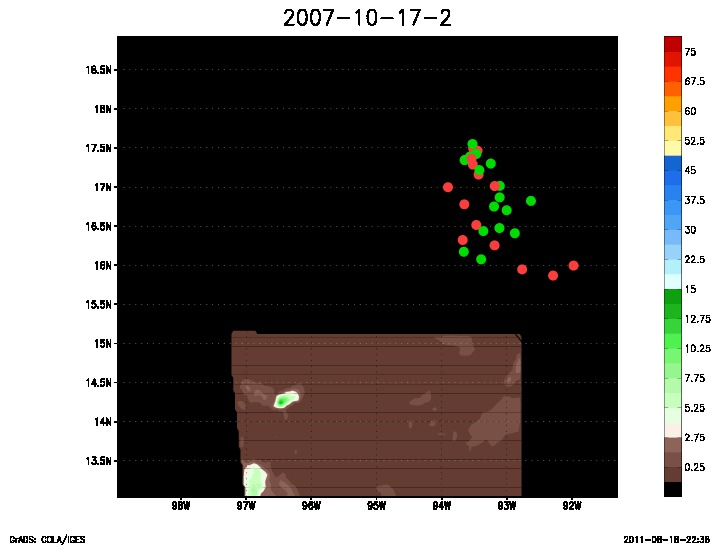
\includegraphics[width=120mm]{./imagenes/2007_10_17_2.jpg}
 % 2007_10_17_01.eps.jpg: 719x555 pixel, 72dpi, 25.36x19.58 cm, bb=0 0 719 555
 \caption{Im'agen generada por GrADS de la ventana completa de datos con informaci'on faltante}
\end{figure}


\section{Dise\~no de la base de datos}

El dise\~no de la base de datos geogr'afica responde a una serie de requerimientos operativos:
\begin{itemize}
 \item Debe guardar cada punto en su contexto espacial y temporal.
 \item Debe guardar la informaci'on de las estaciones de la CFE en su contexto espacial y temporal
 \item Debe guardar la informaci'on de precipitaci'on en cada punto.
\end{itemize}

En la Figura ... se muestra el diseño de la base de datos.

\begin{figure}[h!]
 \centering
 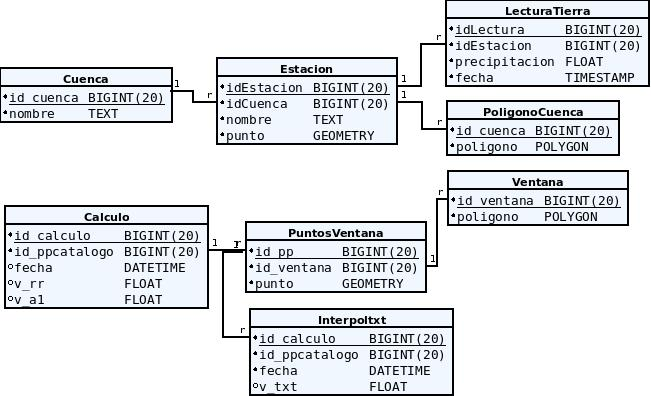
\includegraphics[width=150mm]{./imagenes/DataBase.jpg}
 % DataBase.jpg: 651x396 pixel, 72dpi, 22.97x13.97 cm, bb=0 0 651 396
 \caption{Dise\~no de la Base de Datos Geogr'afica}
\end{figure}

El desempe\~no de la base de datos se ve mejorada ampliamente mediante el uso de 'indices. El incremento en la
velocidad de acceso a la informaci'on se logra mediante la aplicaci'on de 'indices en los campos en donde
se hacen las búsquedas m'as frecuentes.

En 'este proyecto se relizaron 'indices sobre diferentes tablas:
\begin{itemize}
 \item 'Indice sobre el campo \textit{fecha} en la tabla \textit{LecturaTierra}
  \item 'Indice sobre el campo \textit{id\_ventana} en la tabla \textit{PuntosVentana}
  \item 'Indice sobre el campo \textit{fecha} en la tabla \textit{Interpoltxt}
  \item 'Indice sobre el campo \textit{fecha} en la tabla \textit{Calculo}
  \item 'Indice sobre el campo \textit{id\_ventana} en la tabla \textit{Calculo}
  \item 'Indice geogr'afico sobre el campo \textit{punto} en la tabla \textit{Estacion}
  \item 'Indice geogr'afico sobre el campo \textit{punto} en la tabla \textit{PuntosVentana}
\end{itemize}



\section{Dise\~no de la p'agina web}
%Primefaces y JSF
En la actualidad las arquitecturas de software m'as aceptadas y adoptadas en 
el desarrollo web implementan la arquitectura llamada Modelo-Vista-Controlador (MVC).

La arquitectura MVC intenta aislar tres componentes importantes en el desarrollo
de una aplicaci'on web:

\begin{itemize}
 \item \textbf{Modelo:} Administra el comportamiento y los datos de la aplicaci'on mediante peticiones (usualmente de la vista).
\item \textbf{Vista:} Permite acceder e interaccionar con el modelo mediante una interfaz f'acil de usar.
\item \textbf{Controlador: } Recibe entradas del usuario e inicia la respuesta correspondiente haciendo llamadas al controlador.
\end{itemize}

Uno de los marcos de trabajo m'as ampliamente usados que implementan la arquitectura MVC es Java Server Faces (JSF). En JSF las
peticiones del usuario son procesadas por un servidor que carga la vista apropiada, crea el 'arbol de componentes de la vista y
procesa sus eventos. El estado de los componentes de la vista son guardados al final de una petici'on s'incrona o as'incrona al servidor.

El usuario final experimenta una experiencia visual m'as eriquecedora mediante las llamadas as'incronas al servidor que atienden
respuestas en tiempo real en el momento en que se interact'ua con la aplicaci'on. El valor agregado de JSF es la existencia de otros
marcos de trabajo que incrementan la calidad visual de los componentes de la vista, tal es el caso de PrimeFaces.

La p'agina web del presente proyecto se implement'o usando JSF y PrimeFaces para lograr una experiencia visual 'optima
para que la aplicaci'on sea f'acil de usar y atractiva visualmente.

\begin{figure}[!ht]
 \centering
 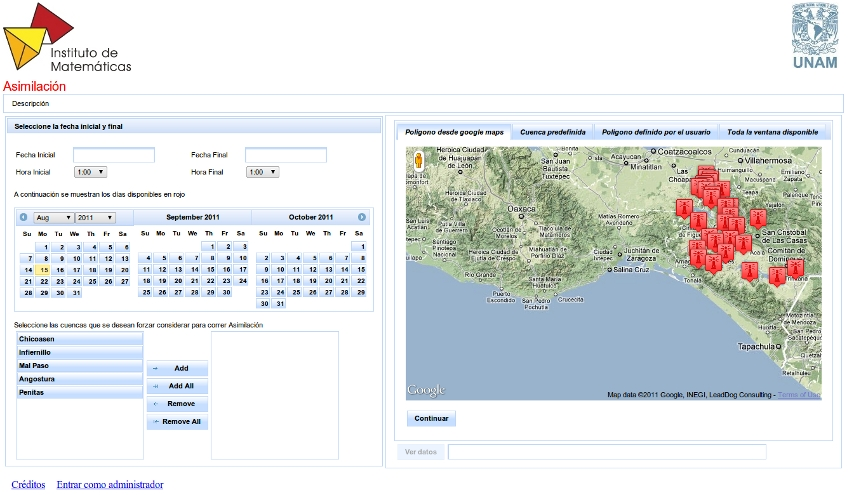
\includegraphics[width=180mm]{./imagenes/pagWeb.jpg}
 % pagWeb.png: 1425x789 pixel, 72dpi, 50.26x27.83 cm, bb=0 0 1425 789
 \caption{http://132.248.17.180:8080/AsimilacionLluvias/}
\end{figure}


La p'agina web permite seleccionar el rango de tiempo en donde se va a ejecutar el algoritmo. Se us'o Google Maps
para ilustrar la distribuci'on geogr'afica de las estaciones y la selecci'on de un poligono definido por el usuario.
La p'agina principal permite al usuario incluir las estaciones de cuencas disponibles para forzar que 
sean consideradas en la correci'on num'erica. 

El sistema requería de un m'odulo de administraci'on de la base de datos geogr'afica que permitiera:
\begin{itemize}
 \item Subir nueva informaci'on satelital.
  \item Subir nueva informaci'on de los mapas de precipitaci'on inicial.
  \item Subir informaci'on de lecturas de estaciones pluviales.
  \item Modificar la informaci'on de las estaciones.
\end{itemize}

La opci'on ideal para implementar 'este m'odulo de administraci'on fue integrarlo a la p'agina web
para que la administraci'on sea posible desde cualquier parte del mundo.


\section{Pruebas de confiabilidad}
%Análisis puntual de los datos de las estaciones
El algoritmo que utiliza los valores de las estaciones de la CFE permite generar un mapa de lluvias dentro de un poligono
determinado. La selección del poligono determina qu'e estaciones se deber'an usar para computar la correcci'on num'erica.

Estas premisas dan pie a analizar de manera puntual como se ha ido corrigiendo las estimaciones pluviales al aplicar
consecutivamente los algoritmos, es decir, mediante interpolaciones num'ericas nos fue posible comparar la precipitaci'on
real reportada por las estaciones de la CFE, contra el resultado del algoritmo STAR y el resultado de la Asimilaci'on.

%%Pensar como se analizarán los resultados (preguntar a antonio)
